\documentclass{standalone}
\usepackage{tikz}
\begin{document}

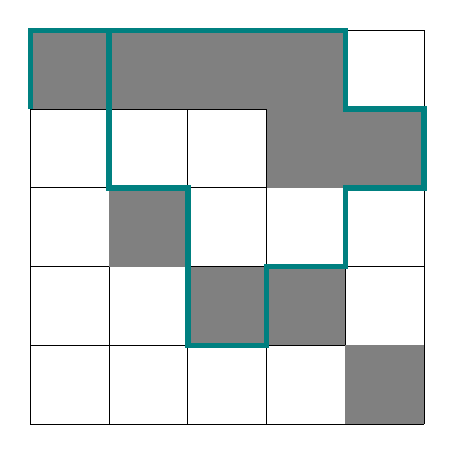
\begin{tikzpicture}
    % Grid
    \draw[step=1cm, black, thin] (0,0) grid (5,5);
    
    % Gray squares
    \fill[gray] (0,4) rectangle (1,5);
    \fill[gray] (1,4) rectangle (2,5);
    \fill[gray] (2,4) rectangle (3,5);
    \fill[gray] (3,4) rectangle (4,5);
    \fill[gray] (3,3) rectangle (4,4);
    \fill[gray] (4,3) rectangle (5,4);
    \fill[gray] (1,2) rectangle (2,3);
    \fill[gray] (2,1) rectangle (3,2);
    \fill[gray] (3,1) rectangle (4,2);
    \fill[gray] (4,0) rectangle (5,1);
    
    % Teal perimeter
    \draw[line width=2pt, teal] 
        (0,4) -- (0,5) -- (4,5) -- (4,4) -- (5,4) -- (5,3) -- (4,3) -- (4,2) -- (3,2) -- (3,1) -- (2,1) -- (2,3) -- (1,3) -- (1,5) -- (0,5) -- (0,4);
\end{tikzpicture}

\end{document}